\documentclass[a4paper,kulak]{kulakarticle}

\usepackage[utf8]{inputenc}
\usepackage[dutch]{babel}

\date{Academiejaar 2017-2018}
\address{
  Informatica \\
  Gegevensbanken \\
  Professor Bettina Berendt\\
  Dr. Bart Bogaerts}
\title{Verslag opdracht 2}
\author{Thomas Bamelis, Michiel Jonckheere, Jaron Maene}

\begin{document}

\maketitle


\section{Deel A}
\begin{enumerate}
		\begin{figure}[!htb]
			\centering
			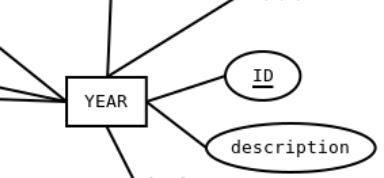
\includegraphics[width=4cm]{verschil1_model}
			\caption{Verschil 1}
			\label{fig:verschil1}
		\end{figure}
	\item Het grootste verschil tussen ons diagram en dat van de modeloplossing is dat wij geen gebruik maakten van een entiteit jaar. Hierdoor zijn enkele gevraagde uitwerkingen bij ons niet mogelijk, zoals het bijhouden van jaarstatistieken van een speler. Dit probleem losten we op door in de assumpties aan te halen dat het enkel mogelijk is om jaarstatistieken af te leiden van de statistieken die een speler had in een team. Deze assumptie is niet zo realistisch, want als een speler in één jaar bij meerdere teams speelt, is het moeilijk jaarstatistieken af te leiden over deze verschillende statistieken van de teams.\\
	In onze uitwerking houden we het jaartal telkens bij als attribuut van een entiteit of relatie. Daardoor zou in onze tabel telkens een extra kolom voor jaartal bijhouden moeten worden. In de modeloplossing zal ofwel het ID van het jaar bijgehouden worden in tabel van de entiteit waarmee het in relatie staat, ofwel zal de relatie zelf een tabel zijn. \\
	Echter was op onze manier het schema wat minder 'spaghetti`.
	
		\begin{figure}[!htb]
			\centering
			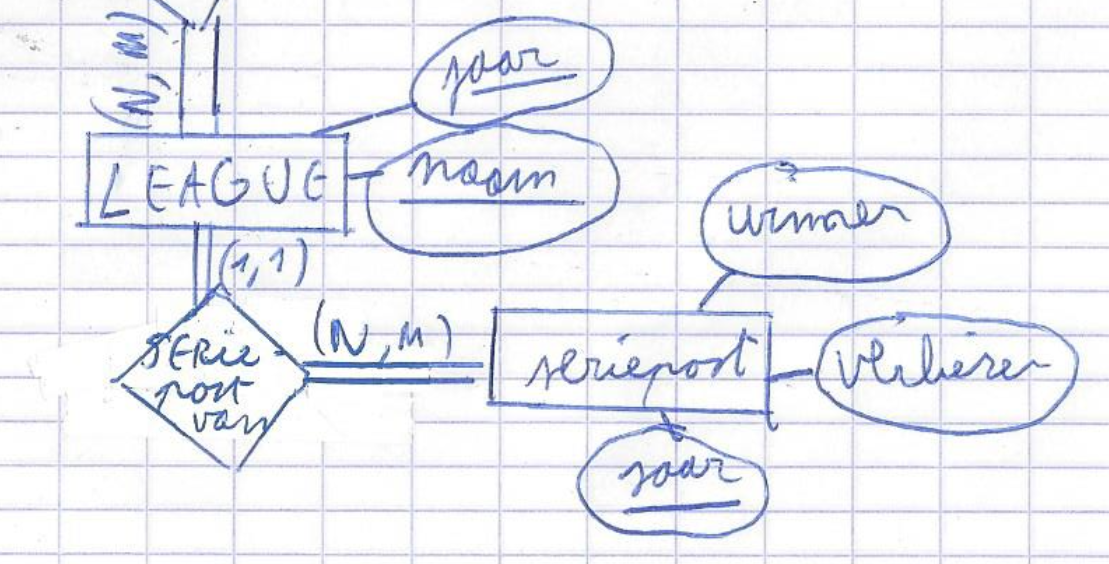
\includegraphics[width=4cm]{verschil2}
			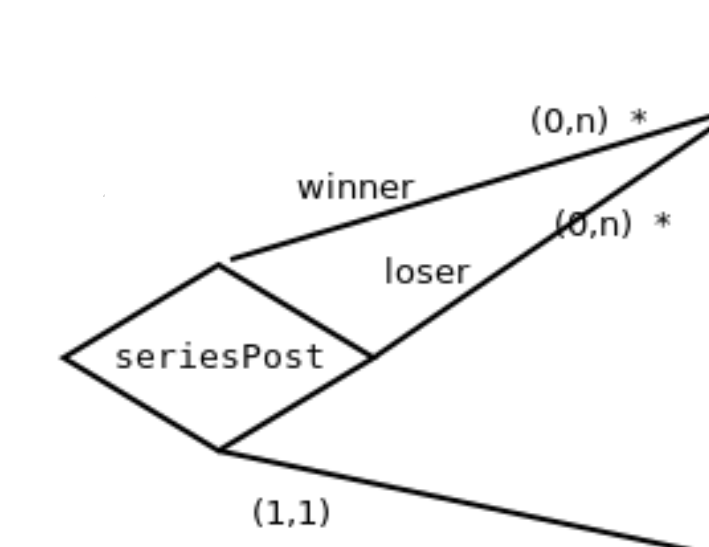
\includegraphics[width=4cm]{verschil2_model}
			\caption{Verschil 2}
			\label{fig:verschil2}
		\end{figure}
	\item Een tweede verschil is de uitwerking van seriespost. Aangezien wij geen entiteit jaar aanmaakten, moesten we dit anders uitwerken. Bij ons heeft elke league een relatie met seriespost, die op zijn beurt per jaar bijhoudt wie de globale winnaar en verliezer is. Hierbij is het wel nodig dat gecontroleerd wordt of het jaar van de league en seriespost telkens overeenkomt. \\
	Het bijhouden van de globale winnaar en verliezer zal in de modeloplossing elk een kolom hebben bij de tabel jaar. Als er met onze oplossing wordt gewerkt, heeft elke league een verwijzing naar de seriespost van zijn jaar. Dit is in principe nogal overbodig en is de uitwerking van de modeloplossing beter.	Als er gewerkt wordt met een entiteit jaar, wordt deze oplossing dus verkozen.
	
		\begin{figure}[!htb]
			\centering
			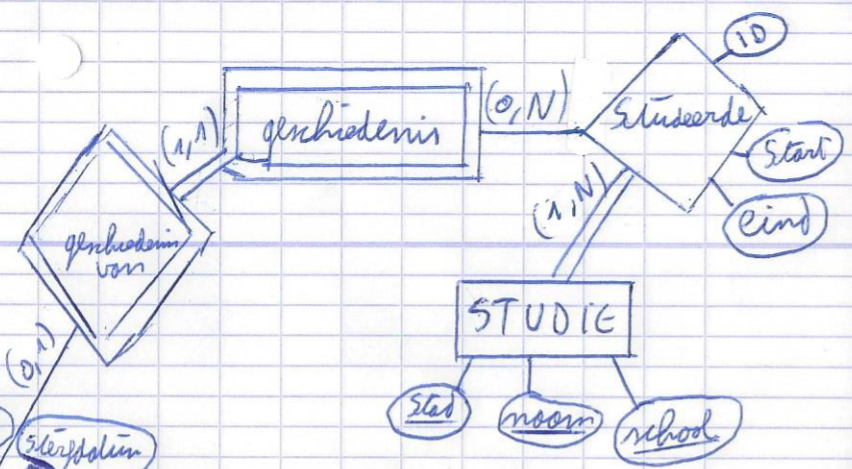
\includegraphics[width=4cm]{verschil3}
			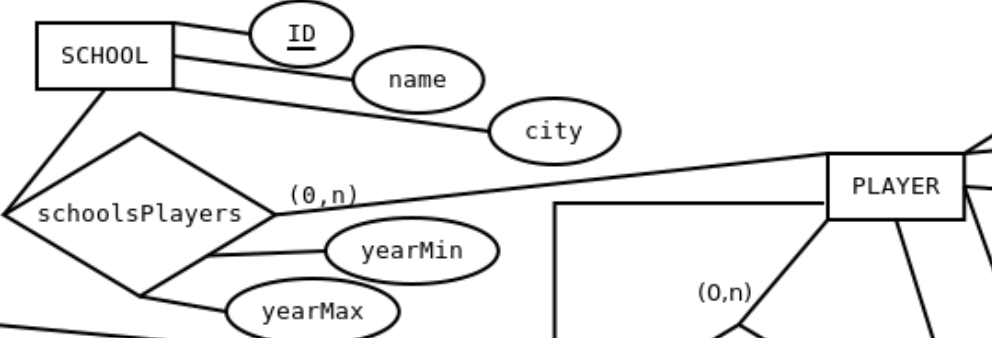
\includegraphics[width=6cm]{verschil3_model}
			\caption{Verschil 3}
			\label{fig:verschil3}
		\end{figure}
	\item In onze uitwerking kozen we voor een zwakke entiteit die de geschiedenis van de speler bijhoudt. Hierdoor is het mogelijk om eventueel nog andere entiteiten aan te maken die hiermee in relatie staan, een voorbeeld kan zijn de medische geschiedenis van de speler. Dit is duidelijk slechter als er geen enkel ander aspect over de geschiedenis werd bijgehouden. Echter werd in de opgave aangegeven dat 'onder andere` de studies werden bijgehouden. Maar zelfs moest er meer bijgehouden worden zou het zelfs nog beter zijn omdat het eigenlijk weinig zin heeft om deze te scheiden. 
	
	
		\begin{figure}[!htb]
			\centering
			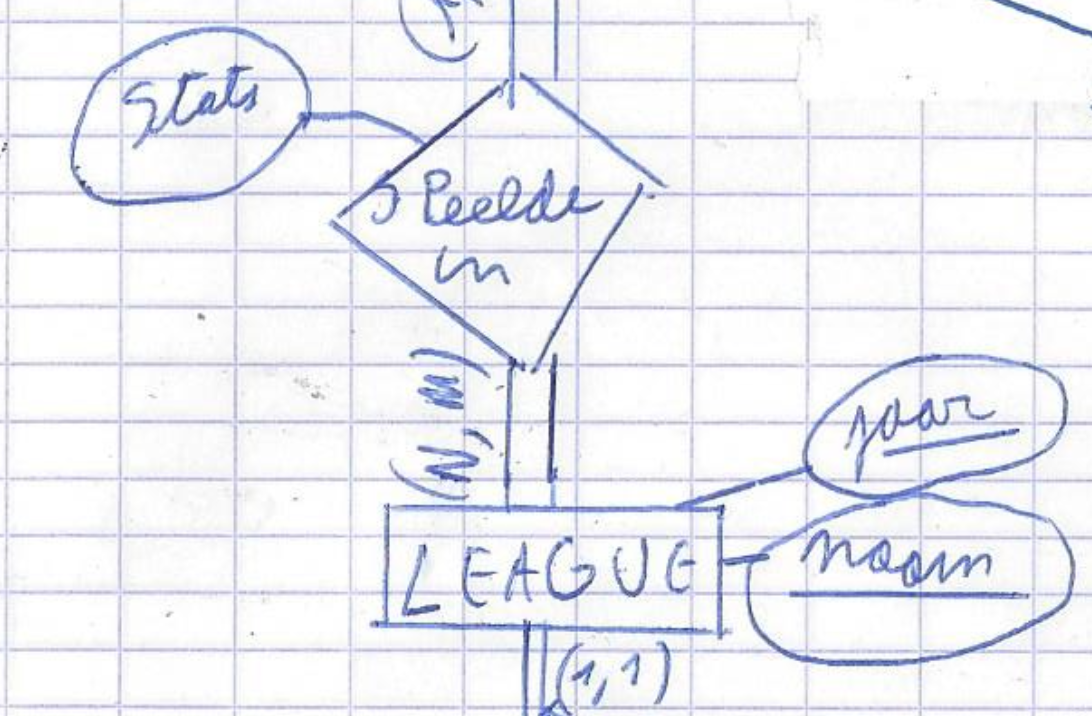
\includegraphics[width=5cm]{verschil4}
			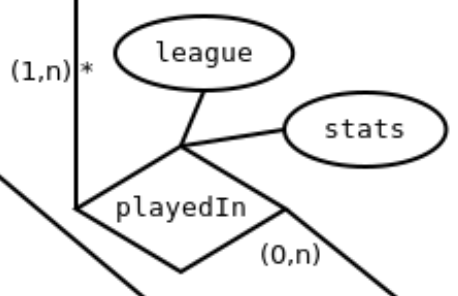
\includegraphics[width=5cm]{verschil4_model}
			\caption{Verschil 4}
			\label{fig:verschil4}
		\end{figure}
	\item Bij het uitwerken van leagues is er ook een verschil. In de modeloplossing is een league enkel een attribuut van de relatie tussen team en jaar. Wij zagen een league als een entiteit die als attribuut dan het jaartal had. 
	League niet als entiteit nemen is minimalistischer en heeft dus de voorkeur.

\begin{figure}[!htb]
	\centering
	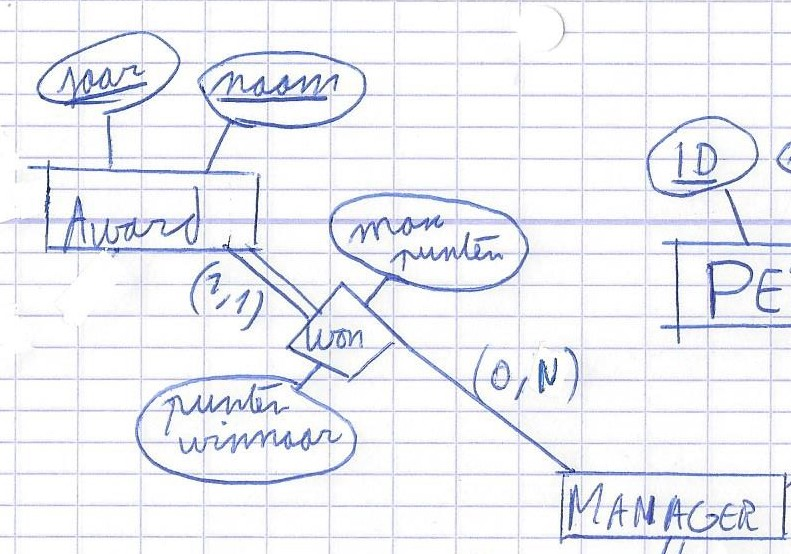
\includegraphics[width=5cm]{verschil5.jpg}
	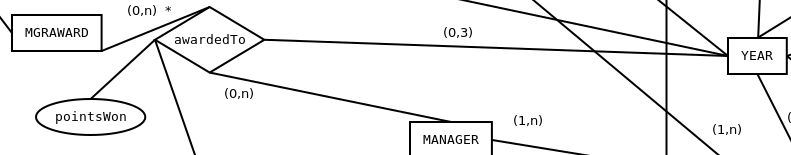
\includegraphics[width=10cm]{verschil5_model}
	\caption{Verschil 5}
	\label{fig:verschil5}
\end{figure}

	\item AwardedTo is in de modeloplossing een ternaire relatie, met het entiteit jaar. Dit is een betere oplossing dan de onze waarbij het jaar werd bijgehouden omdat zo geen 2 primary keys nodig zijn.
	
	
	
\end{enumerate}

\section{Deel B}

\end{document}
